\documentclass[answers]{exam}
\renewcommand{\solutiontitle}{\noindent\textbf{}\par\noindent}

\usepackage{fullpage} % Package to use full page
\usepackage{parskip} % Package to tweak paragraph skipping
\usepackage{tikz} % Package for drawing
\usepackage{amsmath}
\usepackage{blindtext}
%\usepackage{hyperref}
\usepackage{graphicx}
\usepackage{enumerate}
\usepackage{caption}
\usepackage{subcaption}
\usepackage{multicol}
\usepackage{mathptmx}
\usepackage{amsmath}
\usepackage{amssymb}
\usepackage{nameref}
\usepackage{minted}
\usepackage{graphicx}
\usepackage{hyperref}
\hypersetup{
    colorlinks=true,
    linkcolor=blue,
    filecolor=magenta,      
    urlcolor=blue,
}

\newcommand{\mypoints}[1]{\textcolor{red}{(#1 points)}}
\newcommand{\achuta}[1]{\textcolor{magenta}{Achuta: #1}}
\newcommand{\chinmay}[1]{\textcolor{orange}{Chinmay: #1}}
\newcommand{\albert}[1]{\textcolor{purple}{Albert: #1}}
\newcommand{\myinput}[1]{\textcolor{blue}{#1}}

\title{\normalfont \normalsize
\textsc{{Department of Computer Science, UCLA \\
COM SCI 188: Computer Vision}}
\date{\vspace{-12ex}}
}
\begin{document}
\maketitle
\rule{\linewidth}{0.8pt} \\[6pt] 
\noindent
\large\textbf{\textsc{Instructor:}} Prof. Achuta Kadambi, Prof. Stefano Soatto \hfill \large\textbf{\textsc{Name:}} \myinput{Alexander Swerdlow}\\
\large\textbf{\textsc{TAs:}} Aditya Golatkar, Albert Zhao, Chinmay Talegaonkar \hfill 
\large\textbf{\textsc{UID:}} \myinput{305065891}
\rule{\linewidth}{0.8pt} \\[6pt] 

\begin{center}
{\textsc{Homework 4}}\\
1 Late Day Used
\end{center}
% \vspace{2cm}


\begin{table}[h]
\centering
\resizebox{0.8\textwidth}{!}{%
\begin{tabular}{cccc}
\hline
\multicolumn{1}{c}{\textsc{Problem}} &
\multicolumn{1}{c}{\textsc{Type}} &
\multicolumn{1}{c}{\textsc{Topic}} & \multicolumn{1}{c}{\textsc{Max. Points}} \\  \hline \\ 
 \ref{sec:Shape and reflectance} &Analytical & Shape and Reflectance &  10 \\ [2mm]
  2 & Coding & Photometric Stereo &  15 \\ [2mm]
  3 & Analytical & Machine Learning Basics &  10 \\ [2mm]
 4 & Coding & Training a Classifier &  15 \\ [2mm]
 5 & Interview Questions (Bonus) & Miscellaneous &  15 \\  [2mm]
%  [2mm]
    \hline
\end{tabular}
}
\caption*{}
\label{}
\end{table}
\section*{Motivation}
So far we have seen geometric approaches to obtaining 3D features of a scene such as depth and shape. This problem set aims to expose you to a photometric approach to shape estimation, more commonly known as \textit{photometric stereo}. The second half of the problem set gives you a basic exposure to machine learning approaches and techniques used for computer vision tasks such as image classification. You will train a simple classifier network on CIFAR-10 dataset using \href{https://colab.research.google.com/notebooks/intro.ipynb#recent=true}{google colab}. We have provided pytorch code for the classification question, you are free to use any other framework if that's more comfortable.  

The problem set consists of two types of problems: 
\begin{itemize}
    \item analytical questions to solidify the concepts covered in the class, and
    \item coding questions to provide a basic exposure to implementing photometric stereo and building a machine learning classifier using pytorch.
\end{itemize}

\emph{This problem set also exposes you to a variety of machine learning questions commonly asked in job/internship interviews}


\section*{Homework Layout}
The homework consists of 5 problems in total, with subparts for each problem. There are 2 types of problems in this homework - analytical and coding. All the problems need to be answered in the Overleaf document. Make a copy of the Overleaf project, and fill in your answers for the questions in the solution boxes provided. 

For the analytical questions you will be directly writing their answers in the space provided below the questions. For the coding problems you need to use the Jupyter notebooks (see the Jupyter notebook for each sub-part which involves coding). You are provided with 2 jupyter notebooks, for Problem 2 and Problem 4. After writing your code in the Jupyter notebook you need to copy paste the same code in the space provided below that question on Overleaf. In some questions you are also required to copy the saved images (from Jupyter) into the solution boxes in Overleaf. For the classification question, upload the provided notebook to google colab, and change the runtime type to GPU for training the classifier on GPU. Refer to question 4 for more instructions/details. 

\section*{Submission}

You will need to make two submissions: (1) Gradescope: You will submit the Overleaf PDF with all the answers on Gradescope. (2) CCLE: You will submit your Jupyter notebooks (.ipynb file) with all the cells executed on CCLE. 

\section*{Software Installation}

You will need Jupyter to solve the homework. 
You may find these links helpful: 
\begin{itemize}
    \item Jupyter (https://jupyter.org/install)
    \item Anaconda (https://docs.anaconda.com/anaconda/install/)
\end{itemize}

\newpage
\section{Shape and Reflectance}
\label{sec:Shape and reflectance}
\subsection{Plenoptic function \mypoints{1.0}}
How many degrees of freedom does the plenoptic function $L(\boldsymbol{x}, \boldsymbol{\omega}, t, \lambda)$ have. Justify.
\begin{solution}
The plenoptic function has 7 DoF. This is because the equation describes the intensity at a point given a light ray. The equation describes the intensity at a given point $\vec{x}$, the angle of the light ray $\vec{\omega}$ as well as the wavelength $\lambda$ and the time $t$ at which we have the given intensity. The location, $\vec{x}$, can be broken into 3 spatial coordinates $x, y, z$ and the angle of the light ray, $\vec{\omega}$, can be broken into some $\theta, \phi$.  This gives us the full paramaterization of light in space and requires 7 independent variables, hence having 7 degrees of freedom. It is important to note that the light ray can be described in terms of a 3D unit vector but surface normals can be described with only 2 variables.
\end{solution}

\subsection{Lambertian surface \mypoints{3.0}}
At a given pixel $(u, v)$ corresponding to a point on the image of a 3D surface, assume $I(u,v)$ to be the observed intensity, $l$ to the direction of the incident light at the point corresponding to the pixel, and $N(u,v)$ to be a unit vector denoting the surface normal at this point. $N(u,v)$ and $l$ are both $3 \times 1$ vectors. \\    

(i) Assuming a Lambertian surface with an albedo at each point given by $\rho(u,v)$, write an expression for $I(u,v)$. \\

(ii) In above expression, the lighting vector $l$ and the measured intensity $I(u,v)$ is known to us. How many unknown variables we need to solve for at the pixel $(u,v)$? Specify these unknown variables? The 3 components of the normal vector $N(u,v)$ can be denoted as $N_{x}(u,v), N_{y}(u,v), N_{z}(u,v)$. Remember that $N(u,v)$ is a unit vector.  \\

(iii) What is the minimum number of measurements required to solve for the unknown quantities at a given pixel $(u,v)$


\begin{solution}
\begin{enumerate}[i)]
    \item $I(u,v)=\rho(u,v)\cdot l\cdot N(u,v)$
    \item If we know the measured intensity at a given point $I(u,v)$ and the lighting vector $l$, we need to find the surface normal vector $N(u,v)$ as well as the albedo $\rho(u,v)$. Since the surface normal vector has 3 components, $N_{x}(u,v), N_{y}(u,v), N_{z}(u,v)$, and albedo ($\rho(u,v)$) is a real scalar, we initially have these 4 values as unknowns. However, we know that $N(u,v)$ is a unit vector so we only need to solve for $N_{x}(u,v), N_{y}(u,v), \rho(u,v)$ meaning we have \textbf{3 unknowns}.
    \item We have 3 unknowns so we need to take 3 intensity measurements given different lighting vectors to create a system of equations that we can solve.
    \end{enumerate}
\end{solution}

\subsection{Solving Photometric Stereo \mypoints{4.0}} \label{sec:Linearity} 
Having set the stage and notations for photometric stereo in the previous subparts, you will now solve for the unknown surface normals and albedos, thus solving the photometric stereo problem. \\  

(i) Assume that for each pixel $(u,v)$ you obtain $m$ intensity measurements under $m$ different lighting vectors. Let's denote $L$ to be a $m \times 3$ matrix where each row $l$ corresponds to a lighting direction. $I_{m}(u,v)$ denotes a $m \times 1$ vector of the obtained intensity measurements under $L$. Use $G(u,v) = \rho(u,v) N(u,v)$. $G(u,v)$ denotes all the unknowns we are trying to solve for. Obtain $G(u,v)$ as a function of $I_{m}(u,v)$ and $L$. Justify your answer briefly. \\
(ii) Write an expression to obtain $\rho(u,v)$ from $G(u,v)$. \\
(iii) Having obtained $\rho(u,v)$, now derive an expression to obtain $N(u,v)$ from $G(u,v)$. \\  
(iv) Solving the above 2 parts solves the photometric stereo problem for 1 pixel in the image. A naive and inefficient way to scale this up to the whole image is to sequentially apply this operation for each pixel in the image. Let's denote $\hat{N}$ to be a $n \times 3$ matrix, whose each row is the surface normal at a given point on the object surface. We similarly define a $n \times 3$ matrix $\hat{G}$. $n$ is the total number of pixels in the image. Modify your above answers to obtain $\hat{G}, \hat{N}$, thus solving the photometric stereo for the full image in one go. (Assume $I_m$ to be $m \times n$)
\begin{solution}
\begin{enumerate}[i)]
\item From before we have $I(u,v)=\rho(u,v)(L\cdot N(u,v))$
\begin{align*}
I_m(u,v)&=\rho(u,v) l \cdot N(u,v)\\
I_m(u,v)&=L (\rho(u,v)\cdot N(u,v))\\
I_m(u,v)&=L \cdot G(u,v)\\
L^T I_m(u,v)&=L^T L G(u,v)\\
(L^T L)^{-1} L^T I_m(u,v)&=G(u,v)\\
\therefore G(u,v) &= (L^T L)^{-1} L^T I_m(u,v)
\end{align*}
\item Given $G(u,v) = \rho(u,v) N(u,v)$, we also know that $N(u,v)$ is a unit vector. Therefore, $\rho(u,v)$ is equal to the norm of $G(u,v)$:
\begin{align*}
    \rho(u,v) &= ||G(u,v)||\\
\end{align*}

\item Given $G(u,v) = \rho(u,v) N(u,v)$, we have $N(u,v)=\frac{G(u,v)}{\rho(u,v)}=\frac{G(u,v)}{||G(u,v)||}$

\item From (i) we have $G(u,v) = (L^T)^{-1} I_m(u,v)$ 
\begin{align*}
    G(u,v) &= (L^T)^{-1} I_m(u,v) \\
    I_m &= L^T \hat{G(u,v)} \\
    L^T L \hat{G} &= l^T I_m \\
    \hat{G} &= (L^T L)^{-1} L^T I_m
\end{align*}

We then have that for each $n$ row in $\hat{N}$:
\begin{align*}
\hat{\rho} = ||\hat{G}|| \\
\hat{N} = \frac{\hat{G}}{\hat{\rho}}
\end{align*}

\end{enumerate}
\end{solution}
\subsection{Assumptions to be wary of \mypoints{2.0}}\label{sssec:Space_Invariance}
(i) Will the equations derived above work on non-lambertian surfaces? Justify in one sentence. \\ 
(ii) Even for a lambertian surface, can you list 2 scenarios in which the above equations may not give exact results. Assuming no standard photometric stereo assumptions are violated, i.e. the camera is fixed w.r.t object. 

\begin{solution}
\begin{enumerate}[i)]
    \item No, the equations above will not work on non-lambertian surfaces because these equations assume perfectly diffuse reflections which is not the case on non-lambertian surfaces.
    \item One scenario that might perterb the above equations is the case of reflections of light rays. A single light ray may reflect off of several surfaces and hit a single point which would break 
    the assumption that we have a single light ray with a given orientation incident on a point in space. Furthermore, our equations assume that the light source is far from the camera and acts as an ideal light ray which would not be the case given any real light source that is close to the scene.
\end{enumerate}
\end{solution}


\newpage
\section{Implementing Photometric Stereo \mypoints{15.0}} 

In this question you will implement the equations derived in the previous problem, thus implementing photometric stereo. You will be using numpy for this part. Please refer to the given jupyter-notebook for the code setup. Follow the instructions in jupyter-notebook to complete the missing parts. For this part, you will use the notebook named PSET4\_PS. The mathematical notations will be the same used in problem 1.   

\subsection{Loading data \mypoints{4.0}}
(See the jupyter-notebook ) The first step is to images and corresponding lighting vectors for an object. Refer to the corresponding cell (or question) in the jupyter-notebook. In the notebook, we have printed 3 images of the \textsc{cat} object along with the mask. \\

(i) Follow the same template and paste 3 images for the \textsc{bear} object along with its mask in the box below. \\ 
\begin{solution}
    \begin{center}
        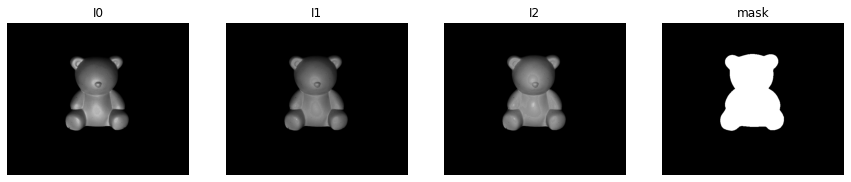
\includegraphics[scale=0.45]{Images/bear.png}
    \end{center}
\begin{minted}{python}
data_dir = '/Users/aswerdlow/Documents/CS188/PSET4/pmsData/'
obj_name =  'bear'
I, L, mask = load_object_data(data_dir = data_dir, obj_name= obj_name)
plt.savefig('Images/bear.png', bbox_inches='tight', facecolor='white')
\end{minted}
\end{solution}
(ii) In the box, paste the code to compute the mean and standard deviation of the magnitude of lighting vectors for all images of a given object. Briefly justify the obtained mean and standard deviation values. \\ 
\begin{solution}
\begin{minted}{python}
L_mean = np.mean(np.linalg.norm(L, axis=-1))
L_std = np.std(np.linalg.norm(L, axis=-1))
print("L_mean : {}, L_std : {}".format(L_mean, L_std))
\end{minted}

\texttt{L\_mean : 1.0000032447074088, L\_std : 2.7981917880143313e-05} \\

We take the mean and std deviation of each of the 96 lighting vectors. Each should have unit norm as they represent the orientation of the lighting vector and we indeed see that the mean is very close to 
$1$ with a very small std deviation suggesting most deviations are a result of finite numerical precision.

\end{solution}
(iii) Write the dimensions of $I_{m}$ and $L$, for the data loaded in the jupyter notebook. Note that $I_{m}$ will be a $m \times n$ matrix where $n$ is the number of pixels in the image. 
\begin{solution}
\begin{minted}{python}
dim_L = L.shape
I_m = I.copy().reshape(96 , I.shape[1] * I.shape[2])
dim_Im = I_m.shape
print("Shape of L: ", dim_L)
print("Shape of dim_Im: ", dim_Im)
\end{minted}
\begin{verbatim}
    Shape of L:  (96, 3)
    Shape of dim_Im:  (96, 313344)
\end{verbatim}
\end{solution}

\subsection{Implementation \mypoints{10}}
You will now implement photometric stereo using the equations derived in problem 1.3. \\

(i) (See the jupyter notebook) Write the code to compute $\hat{G}$ as a function of $I_m$ and $L$ using the expression obtained in (iii) of problem 1.3. 
\begin{solution}
\begin{minted}{python}
H, W = I.shape[1], I.shape[2]
L_inv = np.linalg.pinv(L)
G_hat_vec = np.dot(L_inv, I_m)
G_hat = G_hat_vec.T
\end{minted}

\end{solution}

(ii) (See the jupyter notebook) Write the code to compute a vector $\hat{\rho}$ of size $n \times 1$ which stores the albedo at each pixel. 
\begin{solution}
\begin{minted}{python}
rho_hat = np.linalg.norm(G_hat, axis=-1)
\end{minted}
\end{solution}

(iii) (See the jupyter notebook) Having computed $\hat{G}$ and $\hat{\rho}$, write the code to compute $\hat{N}$. 
\begin{solution} 
\begin{minted}{python}
with np.errstate(all='ignore'):
    N_hat_vec = G_hat_vec / rho_hat
N_hat_vec[np.isnan(N_hat_vec)] = 0
N_hat = N_hat_vec.reshape(3, H, W)
\end{minted}
\end{solution}
(iv) (See the jupyter notebook) In the box below, replace the images shown, and paste the image of the obtained reconstruction, surface normal, and an image showing the error between the two for the \textsc{cat} object. 

\begin{solution}
\begin{center}
    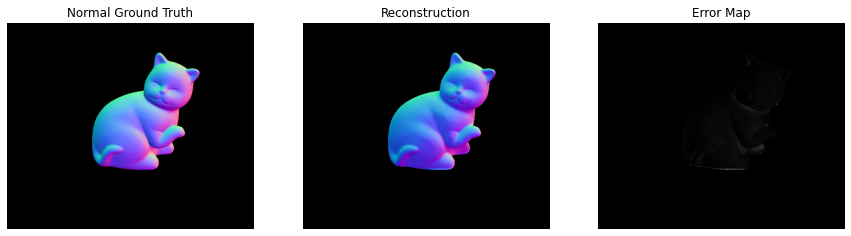
\includegraphics[scale=0.45]{Images/cat.png}
\end{center}
\end{solution}
(v) Repeat part (iv) for the \textsc{ball}, \textsc{reading}, \textsc{pot2}, \textsc{cow} objects.
\begin{solution}
    \begin{center}
        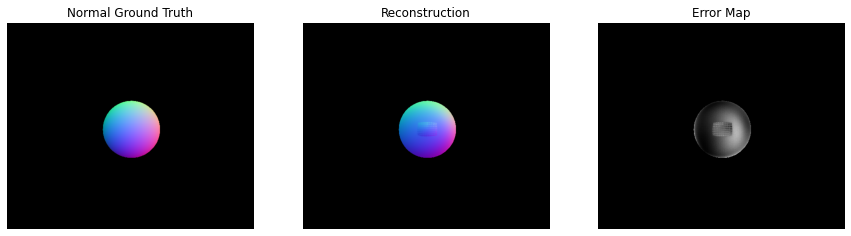
\includegraphics[scale=0.45]{Images/ball.png}
    \end{center}
    \begin{center}
        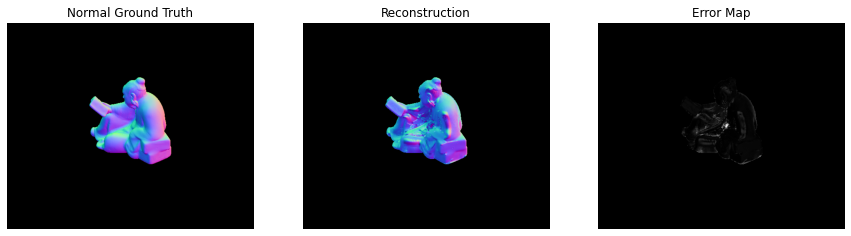
\includegraphics[scale=0.45]{Images/reading.png}
    \end{center}
    \begin{center}
        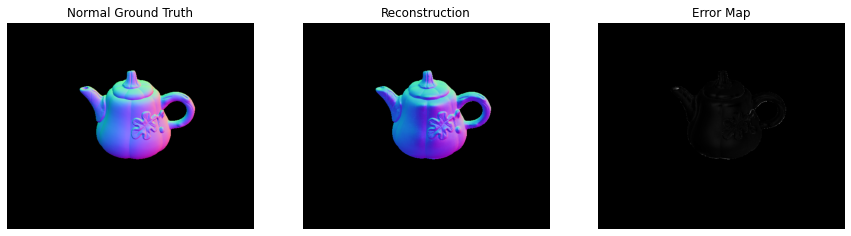
\includegraphics[scale=0.45]{Images/pot2.png}
    \end{center}
    \begin{center}
        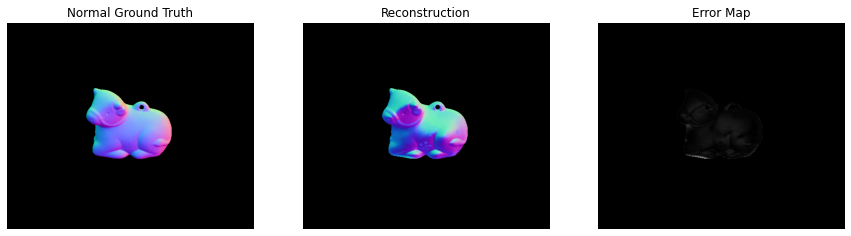
\includegraphics[scale=0.45]{Images/cow.png}
    \end{center}
\end{solution}

\subsection{Qualitative Observation \mypoints{1}}
(vi)You might observe that for some objects, such as \textsc{cat} the error map denotes lower error compared to regions of some objects such as \textsc{ball}. Explain this observation. 
\begin{solution}
This may be because the surface normal has a large gradient on rougher objects, compared to the ball which is smooth, meaning that the normal only changes slightly as you move to a nearby pixel. This may also be caused by inaccurate surface normals being calculated for the object, or because the object is poorly lit in certain areas. For example, it would be difficult to obtain a reconstruction in shadows where there is inadequate light.
\end{solution}

\newpage
\section{Machine Learning Basics \mypoints{10}}
\subsection{Calculating gradients \mypoints{2.0}}
A major aspect of neural network training is identifying optimal values for all the network parameters (weights and biases). Computing gradients of the loss function w.r.t these parameters is an essential operation in this regard (gradient descent). For some parameter $w$ (a scalar weight at some layer of the network), and for a loss function $L$, the weight update is given by $w:=w-\alpha\frac{\partial L}{\partial w}$, where $\alpha$ is the learning rate/step size.

Consider (a) $w$, a scalar, (b) $\mathbf{x}$, a vector of size $(m\times 1)$, (c) $\mathbf{y}$, a vector of size $(n\times 1)$ and (d) $\mathbf{A}$, a matrix of size $(m\times n)$. Find the following gradients, and express them in the simplest possible form (boldface lowercase letters represent vectors, boldface uppercase letters represent matrices, plain lowercase letters represent scalars):
\begin{itemize}
    \item $z=\mathbf{x}^{T}\mathbf{x}$, find $\frac{dz}{d\mathbf{x}}$
    \item $z=Trace(\mathbf{A}^{T}\mathbf{A})$, find $\frac{dz}{d\mathbf{A}}$
    \item $z=\mathbf{x}^{T}\mathbf{A}\mathbf{y}$, find $\frac{\partial z}{\partial\mathbf{y}}$
    \item $\mathbf{z}=\mathbf{A}\mathbf{y}$, find $\frac{d\mathbf{z}}{d\mathbf{y}}$
\end{itemize}

You may use the following formulae for reference:
\begin{equation*}
    \frac{\partial z}{\partial \mathbf{x}}
    =
    \begin{bmatrix}
        \frac{\partial z}{\partial x_{1}}\\
        \frac{\partial z}{\partial x_{2}}\\
        \vdots\\
        \frac{\partial z}{\partial x_{m}}
    \end{bmatrix}
    ,
    \frac{\partial z}{\partial \mathbf{A}}
    =
    \begin{bmatrix}
        \frac{\partial z}{\partial A_{11}} & \frac{\partial z}{\partial A_{12}} & \dots  & \frac{\partial z}{\partial A_{1n}} \\
        \frac{\partial z}{\partial A_{21}} & \frac{\partial z}{\partial A_{22}} & \dots  & \frac{\partial z}{\partial A_{2n}} \\
        \vdots & \vdots & \ddots & \vdots \\
        \frac{\partial z}{\partial A_{m1}} & \frac{\partial z}{\partial A_{m2}} & \dots  & \frac{\partial z}{\partial A_{mn}}
    \end{bmatrix}
    ,
    \frac{\partial \mathbf{y}}{\partial \mathbf{x}}
    =
    \begin{bmatrix}
        \frac{\partial y_{1}}{\partial x_{1}} & \frac{\partial y_{2}}{\partial x_{1}} & \dots  & \frac{\partial y_{n}}{\partial x_{1}} \\
        \frac{\partial y_{1}}{\partial x_{2}} & \frac{\partial y_{2}}{\partial x_{2}} & \dots  & \frac{\partial y_{n}}{\partial x_{2}} \\
        \vdots & \vdots & \ddots & \vdots \\
        \frac{\partial y_{1}}{\partial x_{m}} & \frac{\partial y_{2}}{\partial x_{m}} & \dots  & \frac{\partial y_{n}}{\partial x_{m}}
    \end{bmatrix}
\end{equation*}
\begin{solution}
\begin{enumerate}[i)]
    \item $z=\mathbf{x}^{T}\mathbf{x}$, find $\frac{dz}{d\mathbf{x}}$
    Using $\frac{\partial z}{\partial \mathbf{x}}$ we simplify $\frac{\partial}{\partial \mathbf{x_i}}\sum_{i=1}^{m} x_{i}^{2}=2x_i$ and find that the result is a vector: $2\textbf{x}$. Hence we have: $\frac{dz}{d\mathbf{x}}=2\mathbf{x}$
    \item $z=Trace(\mathbf{A}^{T}\mathbf{A})$, find $\frac{dz}{d\mathbf{A}}$
    Using $\frac{\partial z}{\partial \mathbf{A}}$, we simplify $\frac{\partial}{\partial \mathbf{A_{i,j}}}\sum_{i=1}^{m} \sum_{j=1}^{n} A_{i, j}^{2}=2A_{i,j}$ and find that the result is a matrix: $2\mathbf{A}$. Hence we have: $\frac{dz}{d\mathbf{A}}=2\mathbf{A}$
    \item $z=\mathbf{x}^{T}\mathbf{A}\mathbf{y}$, find $\frac{\partial z}{\partial\mathbf{y}}$
    We again use $\frac{\partial z}{\partial \mathbf{x}}$. We find the derivative as $x^T A$ except we know the result must be (n x 1) so we transpose: $(x^T A)^T = A^T x$. Hence we have: $\frac{\partial z}{\partial\mathbf{y}}=\mathbf{A}^T \mathbf{x}$
    \item $\mathbf{z}=\mathbf{A}\mathbf{y}$, find $\frac{d\mathbf{z}}{d\mathbf{y}}$
    We use the $\frac{\partial \mathbf{y}}{\partial \mathbf{x}}$ formula and find the derivative as simply $\frac{\partial}{\partial\mathbf{y_j}}\sum_{j=1}^{n} A_{i, j} y_{j}=A_j$ which matches the dimensions of $\frac{\partial \mathbf{z}}{\partial \mathbf{y}}$. Hence we have: $\frac{\partial \mathbf{z}}{\partial \mathbf{y}}=\mathbf{A}$
\end{enumerate}
\end{solution}

\subsection{Deriving Cross entropy Loss \mypoints{6.0}}
In this problem, we derive the cross entropy loss for binary classification tasks. Let $\hat{y}$ be the output of a classifier for a given input $x$. $y$ denotes the true label (0 or 1) for the input $x$. Since $y$ has only 2 possible values, we can assume it follow a Bernoulli distribution w.r.t the input $x$. We hence wish to come up with a loss function $L(y, \hat{y})$, which we would like to minimize so that the difference between $\hat{y}$ and $y$ reduces. A Bernoulli random variable (refresh your pre-test material) takes a value of 1 with a probability $k$, and 0 with a probability of $1-k$.  

(i) Write an expression for $p(y|x)$, which is the probability that the classifier produces an observation $\hat{y}$ for a given input. Your answer would be in terms of $y, \hat{y}$. Justify your answer briefly. 
\begin{solution}
\begin{align}
P(y \mid x)&=\left\{\begin{array}{ll}
k & \text { if } y=1 \\
1-k & \text { if } y=0
\end{array}\right. \\
p(y \mid x)&=k^{y}(1-k)^{1-y}\\
% p(y \mid x)&=p(\hat{y}=1)^{y} p(\hat{y}=0)^{1-y}
\end{align}

The probability that we classify some input $x$ as 

\end{solution}
(ii) Using (i), write an expression for $\log p(y|x)$. $\log p(y|x)$ denotes the log-likelihood, which should be maximized.
\begin{solution}
\begin{align}
\log (P(y \mid x)) &=\log \left(k^{y}(1-k)^{1-y}\right) \\
&=\log \left(k^{y}\right)+\log \left((1-k)^{1-y}\right) \\
&=y \log (k)+(1-y) \log (1-k)
\end{align}
\end{solution}
(iii) How do we obtain $L(y, \hat{y})$ from $\log p(x|y)$? Note that $L(y, \hat{y})$ is to be minimized 
\begin{solution}
\begin{align}
L(y, \hat{y}) &=-\log (P(y \mid x)) \\
&=-y \log (k)-(1-y) \log (1-k)
\end{align}
\end{solution}

\subsection{ Perfect Classifier (?) \mypoints{2.0}}

You train a classifier on a training set, achieving an impressive accuracy of 100 \%. However to your disappointment, you obtain a test set accuracy of 20 \%. You bring up this issue in one of the discussions, and the TA suggests some possible steps you could take. For each suggestion below, explain why (or why not) if these suggestions may help improve the testing accuracy.
\begin{enumerate}
    \item Use more training data
    \item Add L2 regularization to your model
    \item Increase your model size, i.e. increase the number of parameters in your model
    \item Create a validation set by partitioning your training data. Use the model with highest accuracy on the validation set, not the training set. 
\end{enumerate}

\begin{solution}
    \begin{enumerate}
        \item This might help improve accuracy if the model has overfitting. With more data we induce more randomness that cannot be captured and thus train to more general solution
        \item This will constrain the weights and prevent us from achieving a "perfect" model in training, since we are not trying to minimize the normal loss, but also the L2 loss. This will result in
        a model that may be less accurate in training but will also likely have less overfitting compared to training without L2 regularization. This is because L2 regularization penalizes the sum of the squares of the weights meaning that larger weights are penalized, leading the model to a more "general" solution.
        \item This might be a good or bad idea depending on the existing model. It may be the case that the existing architecture has too few parameters to properly learn the classes and features and therefore
        has low accuracy. In this case, adding more parameters may allow for more features to be learned. However, oftentimes too many parameters leads the model to overfit the data by memorizing the training set instead of learning the relevant features. If the model is sufficiently complex and the training set is small, the weights may simply overfit to the specific training data and this will result in a poor general solution. Furthermore, adding more parameters invariably increases training time and machine resources so this may not be a good solution.
        \item This will choose a model that has less overfitting as models will not be trained on the validation set so, assuming that the validation set is representative of typical inputs, the model
        with a higher score on the validation set will perform better as a general model. This helps us in choosing a model after training and evaluating its performance, but not with training the model.
    \end{enumerate}
\end{solution}


\newpage

\section{Implementing an image classifier using PyTorch \mypoints{15.0}}
In this problem you will implement a CNN based image classifier in pytorch. We will work with the CIFAR-10 dataset. Follow the instructions in jupyter-notebook to complete the missing parts. For this part, you will use the notebook named PSET4\_Classification. For training the model on colab gpus, upload the notebook on google colab, and change the runtime type to GPU. 

\subsection{Loading Data \mypoints{2.0}}
(i) Explain the function of transforms.Normalize() function (See the Jupyter notebook Q1 cell). How will you modify the arguments of this function for gray scale images instead of RGB images. \\
(ii) Write the code snippets to print the number of training and test samples loaded. 

Make sure that your answer is within the bounding box.
\begin{solution}
The transforms.Normalize() function normalizes the RGB pixel values (the input) to the range [-1, 1]. Since there are 3 color channels here (R/G/B), initially 
with ranges from [0, 1] we need to specify the input for each of the three channels. We need to provide the mean (0.5) of the input channel and the standard deviation (also 0.5) of the input data, so that it can be normalized to the range [-1, 1]. Specifically, Normalize() returns $\frac{value - mean}{std}$, so if we have say a red channel value of 0 initially, we would get $\frac{0 - 0.5}{0.5}=-1$ after
normalization.
\begin{minted}{python}
print(len(train_data))
print(len(test_data))
\end{minted}
There are 50000 training data samples and 10000 test samples loaded.
\end{solution}

\subsection{Classifier Architecture \mypoints{6.0}}
(See the Jupyter Notebook) Please  go  through  the  supplied  code  that defines the architecture (cell Q2 in the Jupyter Notebook), and answer the following questions. 

\begin{enumerate}
\item Describe the entire architecture. The description for each layer should include details about kernel sizes, number of channels, activation functions and the type of the layer. 

\item What does the padding parameter control?

\item Briefly explain the max pool layer.

\item What would happen if you change the kernel size to 3 for the CNN layers without changing anything else? Are you able to pass a test input through the network and get back an output of the same size? Why/why not? If not, what would you have to change to make it work?

\item While backpropagating, we do not need to compute the gradients for the 2 max pooling layers.
\end{enumerate}

\begin{solution}
\begin{enumerate}
    \item The architecture is composed of two convolutional layers, with a max pool operation performed after the first layer. The output of these convolutions are then flattened and passed to a fully connected section composed of 3 layers. Below is a description of each layer.
    
    \begin{itemize}
        \item The first layer takes in the image after all 3 channels have been normalized to a mean and variance of 0.5. The layer performs 3*6=18 convolutions and outputs 6 feature maps, with a kernel size of 5 pixels, a stride of 1, and no padding. Since the kernel is 5x5 and we have no padding, we have an output of 6 feature maps/channels  (result of convolution), each 28x28.
        \item The second layer is a max pooling layer with a 2x2 kernel which means that every 2x2 region for each 6 input channels is turned into a single pixel (max of the 2x2 region). This means we will have an output of 6 channels, each 14x14 (each dimension is exactly half the size as the input dimension).
        \item The 3rd layer (2nd convolution) takes in 6 channels and performs 6*16=96 convolutions to create 16 feature maps/output channels. Each convolution has a 5x5 kernel with a stride of 1 and no padding so the convolution can't be performed at the edges resulting in 16 feature maps output, each 10x10.
        \item The fourth layer is again the same max pooling layer with a 2x2 kernel which means that every 2x2 region for each 16 input channels is turned into a single pixel (max of the 2x2 region). This means we will have an output of 16 channels, each 5x5 (each dimension is exactly half the size as the input dimension).
         \item Next we flatten the output of max pooling (16 5x5 feature maps) into a single vector of length 120. This allows us to pass the data into the fully connected layers.
        \item The first fully connected layer takes in $16*5*5=400$ inputs and has 120 outputs meaning that the layer needs $400 * 120=48000$ weights and 120 biases so each neuron has a weight corresponding to each input (since it is fully connected).
         \item The second fully connected layer has 120 inputs and 84 outputs so it has $120*84=10080$ weights and 84 biases.
        \item The third and last fully connected layer takes in 84 inputs and has 10 outputs meaning that the layer needs $84 * 10 = 840$ weights and 10 biases so each neuron has a weight corresponding to each input (since it is fully connected). This is the last layer of the network and each 10 output values correspond to a classification. To find the 'predicted' class we simply take the max of these 10 values.
      \end{itemize}
      
    
    \item The padding parameter controls how many pixels pad the input to a convolutional layer (default is zero padded). This allows convolution with the outermost pixels that would otherwise need to be 
    ignored because the kernel would not be able to take a dot product with nothing. Without padding, the output size will be smaller than with padding (unless the kernel is 1x1).
    
    \item The max pool layer takes the maximum of a given region, in our network a 2x2 region, and then moves to the next 2x2 region and takes the max, and so on. This provides some invariance to the model because reordering the pixels in that region will produce the same output. This helps to reduce overfitting by giving a more abstract input to future layers and also allows the network to use less paramaters to train as it reduces the input size.
    
    \item If I only changed the kernel size of the convolutional layers, I would not be able to pass a test input through the network because the output of the second max pooling layer will be 16 x 6 x 6 instead of 16 x 5 x 5. This is because both of the convolutional layers will have different output sizes with a 3x3 kernel (30x30 and 13x13 for the 1st and 2nd conv2d layers respectively). To make a 3x3 kernel work, we can change the 1st fully convolutional layer to be: \texttt{self.fc1 = nn.Linear(16 * 6 * 6, 120)}, and change the flattening of our input to: \texttt{x = x.view(-1, 16 * 6 * 6)}.
    
    \item While backpropagating we do not need to compute the gradient to the max pooling layers and the flatten 'layer' because these layers have no parameters to modify and so taking the gradient is meaningless. We still backpropagate through these layers, and specifically, we might need to make note of which pixels that maxpool operation selected so that we can backpropagate beyond the max pool layer, but we do not take the \textit{gradient} of the max pool layer.
    \end{enumerate}
\end{solution}

\subsection{Training the network \mypoints{3.0}}

(i) (See the Jupyter notebook.) Complete the code in the jupyter notebook for training the network on a CPU, and paste the code in the notebook. Train your network for 3 epochs. Plot the running loss (in the notebook) w.r.t epochs. 
\begin{solution}
\begin{minted}[]{python}
## for reproducibility
torch.manual_seed(7)
np.random.seed(7)

## Instantiating classifier
net = Net()

## Defining optimizer and loss function
criterion = nn.CrossEntropyLoss()
optimizer = optim.SGD(net.parameters(), lr=0.001, momentum=0.9)


## Defining Training Parameters

num_epochs = 3 # 2 for CPU training, 10 for GPU training
running_loss_list = [] # list to store running loss in the code below 
for epoch in range(num_epochs):  # loop over the dataset multiple times
    running_loss = 0.0
    for i, data in enumerate(train_loader, 0):
        # get the inputs; data is a list of [inputs, labels]
        inputs, labels = data
        #===============================================#
        # Fill in the training loop here.
        optimizer.zero_grad() # zero the parameter gradients
        outputs = net(inputs) # forward + backward + optimize
        loss = criterion(outputs, labels)
        loss.backward()
        optimizer.step()
        #===============================================#
        # print statistics
        running_loss += loss.cpu().item()
        if i % 250 == 249:    # print every 250 mini-batches
            print('[{}, {}] loss: {:.3f}'.format(epoch + 1, i + 1, running_loss / 250))
            running_loss_list.append(running_loss)
            running_loss = 0.0
            
print('Training Complete')
PATH = './net.pth'
torch.save(net.state_dict(), PATH)
\end{minted}
\end{solution}

(ii) (See the Jupyter notebook.) Modify your training code, to train the network on the GPU. Paste here the lines that need to be modified to train the network on google colab GPUs. Train the network for 20 epochs
\begin{solution}
\begin{minted}[]{python}
net = Net().cuda()

...

outputs = net(inputs.cuda())
loss = criterion(outputs, labels.cuda())

...
\end{minted}
\end{solution}

(iii) Explain why you need to reset the parameter gradients for each pass of the network
\begin{solution}
We need to reset the parameter gradients for each pass using \texttt{optimizer.zero\_grad()} because otherwise the gradients will accumulate for the entire batch and not the "mini-batch." 
This would result in performing regular gradient descent instead of stochastic gradient descent (SGD) which means we would not get the benefit of the noise introduced by computing the gradient with respect to 
mini-batches.
\end{solution}
\subsection{Testing the network \mypoints{4.0}}

(i) (See the jupyter-notebook) Complete the code in the jupyter-notebook to test the accuracy of the network on the entire test set. 
\begin{solution}
\begin{minted}{python}
correct = 0
total = 0
with torch.no_grad():
    for data in test_loader:
        images, labels = data
        outputs = net(images)
        _, predicted = torch.max(outputs.data, 1)
        total += labels.size(0)
        correct += (predicted == labels).sum().item()
acc = correct / total ## stores the accuracy computed in the above loop 
print(f'Accuracy of the network on the 10000 test images: {acc * 100}%')
\end{minted}
\end{solution}
(ii) Train the network on the GPU with the following configurations, and report the testing accuracies and running loss curves -

\begin{itemize}
    \item Training Batch Size 4, 20 training epochs
    \item Training Batch Size 4, 5 epochs
    \item Training Batch Size 16, 5 epochs
    \item Training Batch Size 16, 20 epochs 
\end{itemize}
\begin{solution}

Training Batch Size 4, 20 training epochs — Accuracy 60.74\%
\begin{center}
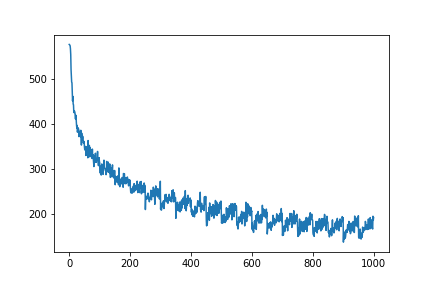
\includegraphics[scale=0.75]{Images/loss-4-20.png}
\end{center}


Training Batch Size 4, 5 training epochs — Accuracy 61.89\%
\begin{center}
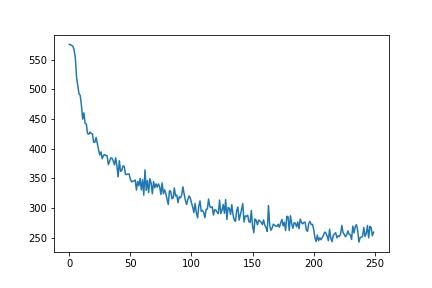
\includegraphics[scale=0.75]{Images/loss-4-5.png}
\end{center}


Training Batch Size 16, 5 training epochs — Accuracy 57.12\%
\begin{center}
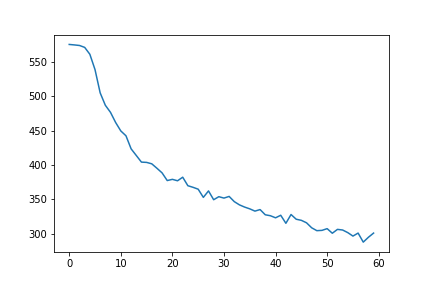
\includegraphics[scale=0.75]{Images/loss-16-5.png}
\end{center}

Training Batch Size 16, 20 training epochs — Accuracy 65.01\%
\begin{center}
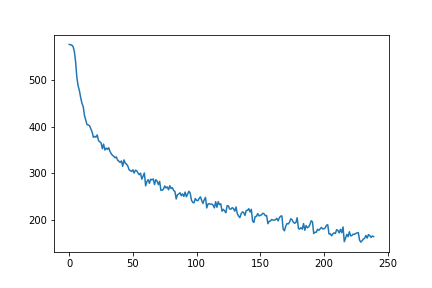
\includegraphics[scale=0.75]{Images/loss-16-20.png}
\end{center}

\end{solution}
(iii) Explain your observations in (ii) 
\begin{solution}
We see that increasing the batch size given a relatively low number of iterations (batch size of 4/16 with 5 epochs) actually decreases the accuracy of the model likely  This is likely due to overfitting that occurs with a larger batch size which increases observed accuracy during training, but decreases the general accuracy of the model as seen during testing. However, given more iterations (batch size of 4/16 with 20 epochs), we see that a larger batch size actually improves accuracy. I believe this occurs because given a sufficient number of iterations, the model encounters a similar amount of noise given fewer iterations but also a smaller batch size. While a larger batch size will introduce less noise into training per iteration, since we have 4x the number of iterations, we likely account for this but also benefit from the gradient being more accurate at each step. A larger batch size makes the gradient more accurate at each step and given a sufficient number of iterations, will outperform a smaller batch size.
\end{solution}

\section{Interview Questions \mypoints{15}}

\subsection{Batch Normalization \mypoints{4}}
Explain \\ 
(i) Why batch normalization acts as a regularizer. \\ 
(ii) Difference in using batch normalization at training vs inference (testing) time. 
\begin{solution}
    \begin{itemize}
        \item Batch normalization acts as a regularizer because it adds noise by normalizing each mini-batch with respect to the calculated mean and covaraince for just that mini-batch and not the entire
        training set. Therefore, this process adds random noise to each layer which provides a regularization effect similar to using dropout. This is because the weights must adjust to be invariant to noise and are therefore more likely to be stable for generalized inputs, preventing overfitting.
        \item The difference between using batch normalization at training vs inference time is that at training time, you want to calculate the mean and varaince with respect to the mini-batch, or possibly a running mean/variance which allows noise to be introduced. However, at inference time, it would likely be a bad idea to normalize with respect to the input data as computing mean/variance for a single input would likely produce an inaccurate result. Therefore, one might use the precomputed mean and variance from training time and apply normalization with respect to those values to ensure consistency of the model.
    \end{itemize}
\end{solution}

\subsection{CNN filter sizes \mypoints{4}}
Assume a convolution layer in a CNN with parameters $C_{in} = 32$, $C_{out} = 64, k = 3$. If the input to this layer has the parameters $C = 32, H = 64, W = 64$. 

(i) What will be the size of the output of this layer, if there is no padding, and stride = 1  \\
(ii) What should be the padding and stride for the output size to be $C = 64, H = 32, W = 32$ 
\begin{solution}
(i) Following the equation provided by PyTorch's Conv2D Function we see that the output size will be 62 x 62:
\begin{align}
H_{out} &= W_{out} = \left \lfloor{\frac{H/W + 2*padding + dilation*(k - 1) - 1}{stride} + 1}\right \rfloor\\
H_{out} &= W_{out} = \left \lfloor{\frac{64 + 2*0 + 1*(3 - 1) - 1}{1} + 1}\right \rfloor = 62
\end{align}

(ii) Again, using the equation provided by PyTorch's Conv2D Function, we see that padding = 1 and stride = 2 will result in H = W = 32:
\begin{align}
H_{out} &= W_{out} = \left \lfloor{\frac{64 + 2*1 + 1*(3 - 1) - 1}{2} + 1}\right \rfloor = 32
\end{align}
\end{solution}

\subsection{L2 regularization and Weight Decay \mypoints{4}}
Assume a loss function of the form $L(y,\hat{y})$ where $y$ is the ground truth and $\hat{y} = f(x,\boldsymbol{w})$. $x$ denotes the input to a neural network (or any differentiable function) $f()$ with paramters/weights denoted by $\boldsymbol{w}$. Adding $L2$ regularization to $L(y, \hat{y})$ we get a new loss function $L'(y, \hat{y}) = L(y, \hat{y}) + \lambda \boldsymbol{w}^{T}\boldsymbol{w}$, where $\lambda$ is a hyperparameter. Briefly explain why $L2$ regularization causes weight decay. Hint: Compare the gradient descent updates to $\boldsymbol{w}$ for $L(y,\hat{y})$ and $L'(y, \hat{y})$. Your answer should fit in the given solution box.
\begin{solution}
L2 regularization causes weight decay because the loss function includes the sum of the squares of the weights in addition to $L(y,\hat{y})$ which penalizes the accuracy of the model. This is a way to penalize the model complexity and prevent overfitting. During backpropagation, the gradient will now account for increased model complexity as larger weights will increase the loss. Therefore, gradient descent updates with L2 regularization will result in smaller weight changes (and smaller weights overall) compared to without regularization.
\end{solution}

\subsection{Why CNNs? \mypoints{3}} 
Give 2 reasons why using CNNs is better than using fully connected networks for image data.
\begin{solution}
One reason why CNNs are better than fully connected networks for image data is that CNNs allow us to preserve structural information that is in the input image while FCNs destroy this data when the image
is flattened into a single vector. CNNs have the ability to learn features that depend on structual information by using convolution and then pass those feature maps to fully connected layers, after those features have already been 'extracted'. Many things that distinguish images such as edges and shapes can be detected using specific kernel filters and so using convolutional layers allows us to train these kernel weights feed only the resulting feature maps to the fully connected layers.

A second important reason to use CNNs over FCNs for image data is that CNNs allow us to use far fewer parameters because convolutional layers only require (feature maps * input channels * k) weights [this calculation ignores biases], while fully connected layers require (input nuerons * layer neurons) weights. However, even a 200x200 image has 40,000 pixels with 3 color channels, resulting in 120 million parameters needed for just 1000 neurons. This is because we need weights for every individual input pixel and channel while convolutional layers allow us to use a small kernel which slides over the image. These kernels allow us to extract information about the image by tuning far fewer parmeters becuase most of the information in an image isn't actually required for tasks such as classification. Hence we can 'compress' it's representation down to feature maps for most tasks. This allows the dense fully connected layers to perform tasks such as classification with far fewer layers and weights.
\end{solution}

% \bibliographystyle{plain}
% \bibliography{bibliography.bib}


\end{document}